\documentclass{bioinfo}
\copyrightyear{2012}
\pubyear{2012}

\usepackage{color}

\begin{document}
\firstpage{1}

% 1139 words w/o abstract and acknowledgements

\title[Data2Dynamics]{Data2Dynamics: a modeling environment tailored to parameter estimation in dynamical systems}
\author[A.~Raue \textit{et~al.}]{A.~Raue\,$^{1,}$\footnote{to whom correspondence should be addressed}, B.~Steiert$^{2}$, M.~Schelker$^{3}$, C.~Kreutz$^{2}$, B.~Sch\"oberl$^{1}$ and J.~Timmer\,$^{2,4,5}$}
\address{$^{1}$Merrimack Pharmaceuticals Inc., 02139 Cambridge, MA, USA\\
$^{2}$University of Freiburg, Institute for Physics, 79104 Freiburg, Germany\\
$^{3}$Humboldt-Universit\"at zu Berlin, Theoretical Biophysics, 10115 Berlin, Germany\\
$^{4}$BIOSS Centre for Biological Signalling Studies, University of Freiburg, 79104 Freiburg, Germany\\
$^{5}$Zentrum f\"ur Biosystemanalyse (ZBSA), University of Freiburg, 79104 Freiburg, Germany}

\history{Received on XXXXX; revised on XXXXX; accepted on XXXXX}

\editor{Associate Editor: XXXXXXX}

\maketitle

\begin{abstract}

\section{Summary:}
Modeling of dynamical systems using ordinary differential equations is a popular approach in the field of Systems Biology. One of the most critical steps in this approach is to conveniently construct dynamical models of biochemical reaction networks for large data sets and complex experimental conditions and to perform efficient and reliable parameter estimation for model fitting. We present a MATLAB based modeling environment that pioneers these challenges. The numerically expensive parts of the required calculations such as the solving of the differential equations and of the associated sensitivity system are parallelized and automatically compiled into efficient C code. A variety of parameter estimation algorithms as well as frequentist and Bayesian methods for uncertainty analysis have been implemented and used on a range of applications that lead to publications. 

\section{Availability and Implementation:}
The Data2Dynamics modeling environment is a collaborative open source project and freely available at %. The code and full documentation are hosted on the website 
\href{http://www.data2dynamics.org}{http://www.data2dynamics.org}. 
%Participation in the further development is highly welcome!

\section{Contact:} \href{andreas.raue@fdm.uni-freiburg.de}{andreas.raue@fdm.uni-freiburg.de}

%Alternativ: (hab ich bei meiner Application Note auch so gemacht)
\section{Supplementary information} {is provided online.} 
%\section{Supplementary information} {A supplementary text with mathematical and numerical details as well as a detailed step-by-step user guide is available.}

\end{abstract}



\section{Introduction}
For the reconstruction of biochemical interaction networks as they occur in signal transduction or gene regulation, data sets generated under a wide range of experimental conditions have to be analyzed comprehensively.
Here a software implementation is presented which is designed for efficient and convenient fitting of ODE models and offers great flexibility for specifying complex relationships between data sets and inferred dynamical model.


%The dynamics of cellular processes such as signal transduction or gene regulation can be described by models consisting of coupled non-linear ordinary differential equations (ODE). 
%For the reconstruction of biochemical interaction networks, data sets generated under a wide range of experimental conditions have to be analyzed comprehensively.
%Here a software implementation is presented which is designed for efficient and convenient fitting of ODE models offers great flexibility for specifying complex relationships between data sets to inferred dynamical model.
% nonlinear ??

\section{Methodology}
%\paragraph{Model Construction}
%Mathematically, such dynamical systems can be characterized by 
%\begin{equation}
%{\bf \dot  x}(t,{\boldsymbol \theta}) = {\bf f}({\bf x}(t,{\boldsymbol \theta}),{\bf u}(t,{\boldsymbol \theta}),{\boldsymbol \theta})
%\quad \textnormal{with} \quad {\bf x}(0,{\boldsymbol \theta}) = {\bf g}(\boldsymbol{\theta}).
%\label{eq:ode}
%\end{equation}
%${\bf \dot  x}(t,{\boldsymbol \theta}) = {\bf f}({\bf x}(t,{\boldsymbol \theta}),{\bf u}(t,{\boldsymbol \theta}),{\boldsymbol \theta})$
%with ${\bf x}(0,{\boldsymbol \theta}) = {\bf g}(\boldsymbol{\theta})$. In this case the vector of state variables ${\bf x}(t,{\boldsymbol \theta})$ describes the dynamics of molecular components. The function ${\bf u}(t,{\boldsymbol \theta})$ represents experimental treatments that are time-varying inputs to the ODE systems.
Our software allows to directly specify the right hand side of the ODE manually, or to automatically generate it by  providing a reaction scheme such as $A + B \rightarrow C$ with the respective rate-law like Mass Action or Michaelis-Menten. 
%In the latter case, for specifying the reaction rate equations one can either choose to apply default Mass Action kinetics, either reversible $\leftrightarrow$ or non-reversible $\rightarrow$, or a custom rate law such as Michaelis-Menten or Hill kinetics. 
The resulting ODE system as well as its Jacobian matrix that is calculated automatically by symbolic differentiation are translated to C code and complied together with the ODE solver. %In case of 2), t
The code makes efficient use of pre-calculated reaction fluxes as described in the Supplementary Information~1. 
Time-varying inputs to the ODE systems can be represented by custom or predefined input functions such as steps, pulses and splines that can depend on unknown parameters \citep{Schelker:2012uq}. 
The initial concentrations %${\bf x}(0,{\boldsymbol \theta})$ 
can be considered as functions %${\bf g}(\boldsymbol{\theta})$ 
of unknown parameters as well. 
%For a specific cell type or biological context, the unknown parameters %${\boldsymbol \theta}$ 
%are often not available  from literature and have to be estimated from experimental data. 
The software allows considering multiple different models that can share common parameters and fit them simultaneously to all available data. 

A unique feature of the Data2Dynamics software is its ability to consider and estimate the magnitude of measurement errors.
%\paragraph{Dataset and Experimental Conditions}
Observations are only required for a subset of all dynamic states and experimental data %provides information to estimate unknown model parameters by fitting the model. 
%Each possible measurement is mathematically represented by a functional mapping
%%\begin{equation}
%%    {\bf y}(t,{\boldsymbol \theta}) = {\bf h}({\bf x}(t,{\boldsymbol \theta}),{\bf u}(t,{\boldsymbol \theta}),{\boldsymbol \theta}). \label{eq:obs}
%%\end{equation}
%${\bf y}(t,{\boldsymbol \theta}) = {\bf h}({\bf x}(t,{\boldsymbol \theta}),{\bf u}(t,{\boldsymbol \theta}),{\boldsymbol \theta})$
%that and 
might include additional parameters such as scaling or offset parameters.% and thus increase the dimension of ${\boldsymbol \theta}$. 
%Not all state variables have to occur in ${\bf y}$, thus the system
%can be only partially observed. %For each model, multiple datasets can and should be considered simultaneously. 
Another key feature of the Data2Dynamics software is its ability to conveniently and automatically create model variants that represent different experimental conditions. These conditions can be defined directly in the data sheets that contain the measurements and are conveniently parsed and grouped. 
For instance, a time course experiment 
with all combinations of two treatment options
automatically yields four experimental conditions
of the ODE system linked to the respective data. 
The model simulation will be plotted in the same grouping as well, see trajectories in different color in Fig.~1. %Another frequently occurring case are 
For dose response experiments, %at fixed time points. In this case 
the software again automatically generate all required model variants and display the simulation results in a dose response plot. For computational efficiency, experimental conditions, and thus model variants, that are shared between different experiments are calculated only once. Since all variants of the original ODE system have to be solved independently, the C code automatically parallelizes the execution of the ODE solver, see Supplementary Information~3 for a performance comparison. 

%\paragraph{Experimental Noise}
%Another unique feature of the Data2Dynamics software is its ability to consider and estimate uncertainty in experimental data. Using the full Likelihood function, see Supplementary Information~4 for details, we demonstrated that this approach provides a robust and reliable determination of experimental noise \citep{Raue:2012zt}. The software is able to estimate the amount of experimental noise simultaneously with the unknown parameters that define the dynamics, see shades around trajectories in Fig.~1. A determination of measurement noise by manual inspection or by a preprocessing procedure is not required any more. Therefore, the results that are obtained by our software are independent of the degree of the experimenter's believe in the quality of the experimental data.
\begin{figure}[!tpb]%figure1
\centerline{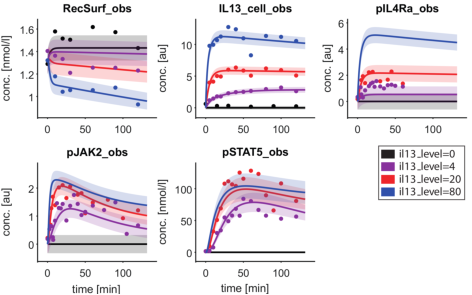
\includegraphics[width=\linewidth]{Figure_D2D_AppNote_v2a.pdf}}
\caption{\citet{Raia:2011vn} model fitted to experimental data (dots) representing four different doses of IL-13. The solid lines are the the fitted model trajectories, the shades the estimated experimental noise levels of the data. A detailed step-by-step user guide for this example can be found in the Supplementary Information~2.}\label{fig:01}
\end{figure}
%\paragraph{Parameter Estimation}
A critical task in modeling of dynamical systems is the efficient and reliable estimation of model parameters, also called model fitting. We implemented a variety of different parameter estimation algorithms \citep{Raue:2012zt}. The most efficient and reliable algorithm for parameter estimation in our hands is a deterministic trust region approach combined with multi-start strategy to map out local minima. Parameters can and should be estimated on a log-scale. %For experimental data, the software allows to compare model to data on a log scale as well. 
Prior knowledge about the parameters can be considered as well. 
If steady state assumptions %${\bf \dot  x}(t) = 0$ 
for the model dynamics are required and the functional relationship to parameters are unknown, %, and its solution %${\bf g}(\boldsymbol{\theta})$ is not known, 
steady state constraints can be added to the objective function, including the respective derivatives. A quality control, as proposed in \citet{Raue:2012zt} can be performed to validate robustness of the estimation results.

%\paragraph{Sensitivity Equations}
The software implements a sophisticated method to calculate model sensitivities, i.e.~the derivatives of the dynamics with respect to model parameters, see Supplementary Information~5 and 6 for details. The sensitivity equations are derived automatically by symbolic differentiation, translated to C code and complied together with the original ODE systems and the solver. We showed previously \citep{Raue:2012zt} that this approach is not only about ten times faster but also more precise than the default approach using finite differences. A reliable calculation of these derivatives is key to successful parameter estimation. 

%\paragraph{Uncertainty Analysis and Experimental Design}
In addition to finding the best model fit to a given collection of data, the Data2Dynamics software implements a wide range of algorithms that are able to determine uncertainties in the estimated parameter as well as in the predicted model dynamics. In particular, the frequentist profile likelihood approach for identifiability analysis \citep{Raue:2009ec}, the prediction profile likelihood approach for observability analysis \citep{Kreutz:2011kx} as well as a variety of Bayesian approaches \citep{Raue:2013fk, Hug:2012fk} that calculate posterior probability distributions are available. Based on the results of such uncertainty analyses, the software allows to design additional experiments \citep{Steiert:2012fk} that can resolve non-identifiability and non-observability \citep{Raue:2010fk, Kreutz:2013uq} and improve prediction accuracy.

%\paragraph{Visualization and Reports}
%A variety of automatically generated plots and visualizations of all simulated quantities as well as experimental data, model structure and parameter estimation and uncertainty analysis results are available. All information about the model equations, the data set and estimation results as well as generated figures can be automatically complied into a Latex based PDF report.

\section{Summary}
We present the Data2Dynamics software, a modeling environment that is especially tailored to parameter estimation and model fitting in dynamical systems. The code is open source and is developed in a community effort using a web-based hosting service and a revision control system. A variety of published applications, e.g.~\citet{Becker:2010hs, Raia:2011vn, Bachmann:2011fk}, that made use of the software are provided as benchmark examples for further methods development and as guide for novel applications. For these examples not only the models but also all datasets and their link to the models as well as all original information used in the parameter estimation and uncertainty analysis are provided. The software was awarded twice as best performer in the Dialogue for Reverse Engineering Assessments and Methods (DREAM, 2011 and 2012).

\section*{Acknowledgement}
We thank all academic and industrial collaborators that helped to evolve this modeling environment, in particular the Timmer group at the University of Freiburg, the Klingm\"uller group and the H\"ofer group at DKFZ Heidelberg, the Theis group at the German Research Center for Environmental Health, the Bode group at the University Hospital of D\"usseldorf, the Klipp group at the Humboldt-University Berlin, Merrimack Pharmaceuticals in Cambridge as well as the Shvartsman lab at Princeton. 
%
%\paragraph{Funding\textcolon} 
This work was supported by the German Ministry of Education and Research (LungSys2 0316042G, Virtual Liver Network 0315766, ViroSign 0316180A).

\paragraph{Confict of interest\textcolon} None declared.

\bibliographystyle{natbib}
\bibliography{/Users/araue/Sites/pub/bibtex/Library}

\end{document}